%%% INTRODUCTION AND BACKGROUND
\chapter{INTRODUCTION AND BACKGROUND}
\label{chap:intro}

%%% OVERVIEW
\section{Overview}
The goal of image classification or image recognition is to classify images based on contextual information present in the image. It is the task of assigning an input image a label from a fixed set of categories. Computer vision and machine learning based methods have been used to find solutions to this problem. Challenges in this problem consist of viewpoint variation, scale variation, rotation variation, inconsistent illumination and intra - class variation among others. More recently, deep learning methods known as convolutional neural networks have produced very good results on large scale image datasets. These datasets like Imagenet \cite{deng2009imagenet} consist of natural images consisting of multiple images of objects that occur in everyday life. Image datasets analysed in this thesis consist of images in the scientific domain. Scientific images are usually imaged using sophisticated instruments like microscopes, MRI scanners, X-rays. In addition to the challenges in natural image classification, additional challenges in scientific images include data imbalance, noisy images and  occlusion. The number of images in the dataset are usually small in number. As a result, image classification in the scientific domain comes with it's unique set of problems. 
Image classification systems in scientific domains are usually organized as pipelines or workflows. An example of such a workflow is shown in Fig.  \ref{fig:flowchart1}

\begin{figure}[ht!]
    \centering
    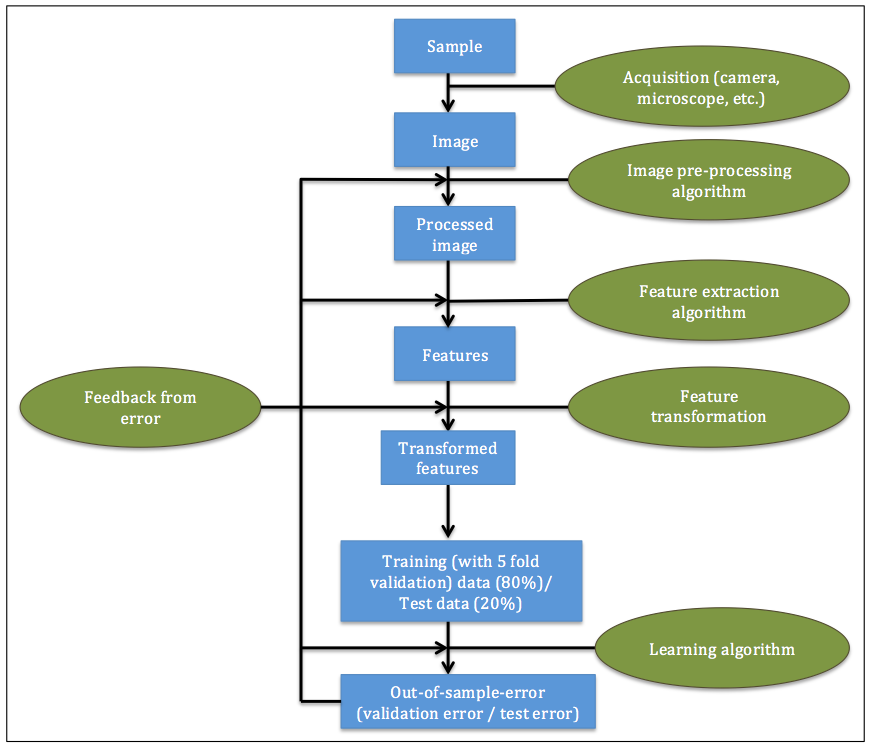
\includegraphics[scale=0.7]{img/EP/flowchart}
    \caption{Representation of an image classification pipeline}
\label{fig:flowchart1}
\end{figure}

The flowchart starts with a sample that is imaged with acquisition technology like a camera or a microscope. The image is then processed using image pre-processing algorithms like normalization and standardization. This may also include image segmentation algorithms. This is followed by feature extraction algorithms that extract useful information from the images. Sometimes, the features extracted are transformed to a different vector space using feature transformation (feature selection or dimensionality reduction) algorithms. The dataset is then divided into training and test datasets in an 80-20 split. Finally, learning algorithms like random forests and logistic regression are used as learning algorithms to build a predictive model for the image classification problem. The performance of the pipeline is evaluated using classification metrics like cross-entropy loss, F1-score, accuracy, precision and recall.  The error in the image classification pipeline maybe measured by such metrics. In this thesis, we base our work on variations of this workflow. Even though the error in image classification pipelines are observed only in terms of the classification error, the source of the error is not just the classification algorithms. The final error is a result of the accumulation of error starting from the beginning of the pipeline right down to the learning algorithms used for classification. Therefore, attempts at improving the performance of image classification pipelines involve the use of  better components in the workflow. This includes using better algorithms and methods for performing data analysis on the image datasets. It may also include improving the quality of the image dataset themselves. Another approach  is to optimize and minimize the error from the pipeline by optimizing the data analytic portion of the pipeline as a whole. This could mean searching the solution space of algorithms to find the best set of algorithms for a particular problem. 
There is also a lack of interpretability of such image classification pipelines, in terms of understanding the source of the errors in the image classification pipeline pertaining to a particular dataset. 
 In this thesis, we present approaches for reducing and quantifying the error in image classification with respect to scientific image datasets from different domains. These methods maybe used by domain experts or scientists to train high quality image classification pipelines for similar datasets.  In addition, we also propose methods to quantify the error from all the components of a machine learning pipeline. These methods maybe used by domain experts and data scientists alike to understand and interpret results from image classification pipelines.  

%%% CONTRIBUTIONS
\section{Contributions}
We made the following contributions over the coarse of four projects discussed in the following chapters:
\begin{enumerate}

\item We report an automated method for characterization of microvessel morphology by performing data augmentation using parametric 3D models of neuropathological blood vessels. We show that a combination of natural and artificial data perform better in terms of classification metrics.  We propose the development of parametric 3D models of blood vessels and this is used to augment datasets for two classification tasks that involve the classification of morphology of blood vessels. They consist of the classification between singular blood vessels and double blood vessels, and between vessels that consist of lumen and those that don't.

\item We perform an exhaustive search of data analytic algorithms in the problem of microstructure recognition. The steps included in this work include feature extraction, feature selection and classification algorithms. Each step consists of various algorithms. Two binary image classification tasks are performed in this work. They consist of classification between dendritic and non-dendritic microstructures and between longitudinal and transverse dendrites. We show that this methodology can be used to identify the best configuration of algorithms and hyperparameters in the domain of microstructure recognition.
An exhaustive grid search on the pipeline also shows that pre-trained convolutional neural networks maybe used to represent images of microstructures in the domain of material science.

\item We propose an automated machine learning based score to quantify the quality of an image. This method maybe used to filter a dataset based on the quality of the images. This method can be used by domain experts to perform data analysis on a dataset that only consists of images with a high amount of signal. It can also be used to quantify the quality of an entire dataset or the quality of a protein marker for analysis.

\item We propose an \textit{agnostic} methodology to quantify the contribution of errors from different components of an image classification pipeline. 
We show empirically that performing random search on the entire pipeline maybe used for accurately and efficiently computing the statistics of error contribution from computational steps, algorithms and hyperparameters in an image classification pipeline.

\end{enumerate}

%%% OUTLINE
\section{Outline}
The following chapters detail our contributions with respect to reduction and quantification of error in image classification pipelines.
In Chapter \ref{chap:ISBI}, we propose a parametric 3D model based data augmentation method used in classification of morphologies of blood vessels in neuropathological tissue samples. 
In Chapter \ref{chap:COMMAT}, we boxdescribe the problem of microstructure recognition with respect to two classification tasks. 
In Chapter \ref{chap:SPIE1}, we present a machine learning based \textit{Quality of Image} score that can automatically quantify the quality of an image or an image dataset.
In Chapter \ref{chap:EP}, we propose and describe a methodology to quantify the contributions of error from different components of an image classification pipeline. 
In Chapter \ref{chap:conclusions} we present summarized conclusions and discuss relevant future
work. 